\documentclass[11pt]{article}

%% Separate file for preamble with macros and stuff
\usepackage[T1]{fontenc}
\usepackage[a4paper, top=1in, bottom=1.1in, left=1in, right=1in]{geometry}
\usepackage[toc,page]{appendix}
\usepackage[utf8]{inputenc} % utf8
\usepackage{amsmath}
\usepackage{attachfile}
\usepackage{booktabs}
\usepackage{caption}
\usepackage{commath}
\usepackage{graphicx}
\usepackage{hyperref}
\usepackage{listings}
\usepackage{mathtools}
\usepackage{siunitx}
\usepackage{subcaption}
\usepackage{tabularx}
\usepackage{url}
\usepackage{varioref}
\usepackage{wrapfig}
\usepackage{xcolor}

\setlength{\belowcaptionskip}{-6pt}
\makeatletter
\lst@Key{matchrangestart}{f}{\lstKV@SetIf{#1}\lst@ifmatchrangestart}
\def\lst@SkipToFirst{%
  \lst@ifmatchrangestart\c@lstnumber=\numexpr-1+\lst@firstline\fi
  \ifnum \lst@lineno<\lst@firstline
  \def\lst@next{\lst@BeginDropInput\lst@Pmode
    \lst@Let{13}\lst@MSkipToFirst
    \lst@Let{10}\lst@MSkipToFirst}%
  \expandafter\lst@next
  \else
  \expandafter\lst@BOLGobble
  \fi}
\makeatother

\lstset{  
  backgroundcolor=\color{gray!30},   % choose the background color; you must add \usepackage{color} or \usepackage{xcolor}
  basicstyle=\scriptsize,        % the size of the fonts that are used for the code
  breakatwhitespace=false,         % sets if automatic breaks should only happen at whitespace
  breaklines=true,                 % sets automatic line breaking
  captionpos=t,                    % sets the caption-position to bottom
  escapeinside={\%*}{*)},          % if you want to add LaTeX within your code
  extendedchars=true,              % lets you use non-ASCII characters; for 8-bits encodings only, does not work with UTF-8
  frame=single,                   % adds a frame around the code
  keepspaces=true,                 % keeps spaces in text, useful for keeping indentation of code (possibly needs columns=flexible)
  keywordstyle=\color{blue},       % keyword style
  language=C++,                 % the language of the code
  numbers=left,                    % where to put the line-numbers; possible values are (none, left, right)
  numbersep=20pt,                   % how far the line-numbers are from the code
  numberstyle=\tiny\color{gray}, % the style that is used for the line-numbers
  rulecolor=\color{blue!20},       
  showspaces=false,                % show spaces everywhere adding particular underscores; it overrides 'showstringspaces'
  showstringspaces=false,          % underline spaces within strings only
  showtabs=false,                  % show tabs within strings adding particular underscores
  stepnumber=1,                    % the step between two line-numbers. If it's 1, each line will be numbered
  tabsize=2,                   % sets default tabsize to 2 spaces
  framesep=7pt,
  xleftmargin=12pt,
  xrightmargin=11pt
}


\setlength{\fboxsep}{4pt}
\DeclareCaptionFormat{myformat}{%
  \hspace{1pt}\fcolorbox{blue!20}{gray!20}{\footnotesize\parbox{\dimexpr\textwidth-17pt\relax}{#1#2\ttfamily#3}}\vspace{-4pt}
}
\captionsetup[lstlisting]{format=myformat}

\captionsetup[figure]{labelfont=sf,hypcap=false,format=hang,margin=0.5cm,justification=RaggedRight,calcwidth=0.7\linewidth,font=footnotesize,justification=justified}
\captionsetup[subfigure]{labelfont=sf,hypcap=false,format=hang,margin=0.5cm,justification=RaggedRight,calcwidth=0.7\linewidth,font=footnotesize,justification=justified}
\captionsetup[table]{labelfont=sf,hypcap=false,format=hang,margin=1cm,justification=RaggedRight,calcwidth=0.8\linewidth,font=footnotesize,justification=justified}
\labelformat{equation}{(#1)}

%%% Math typesetting macros
\newcommand{\di}[2]{#1_\textup{#2}} % Descriptive Index: Macro for quick upright index (as opposed to a variable index, which should be italic)


\renewcommand{\lstlistlistingname}{Code listings}
\bibliographystyle{ieeetr}


%%%%%%%%%%%%%%%%%%%%%%%%%%%%%%
%%% STOLEN FROM STACKOVERFLOW
%%%%%%%%%%%%%%%%%%%%%%%%%%%%%%

\newcommand\YAMLcolonstyle{\color{red}\mdseries\scriptsize}
\newcommand\YAMLkeystyle{\color{black}\bfseries\scriptsize}
\newcommand\YAMLvaluestyle{\color{blue}\mdseries\scriptsize}

\makeatletter

% here is a macro expanding to the name of the language
% (handy if you decide to change it further down the road)
\newcommand\language@yaml{yaml}

\expandafter\expandafter\expandafter\lstdefinelanguage
\expandafter{\language@yaml}
{
  keywords={true,false,null,y,n},
  keywordstyle=\color{darkgray}\bfseries,
  basicstyle=\YAMLkeystyle,                                 % assuming a key comes first
  sensitive=false,
  comment=[l]{\#},
  morecomment=[s]{/*}{*/},
  commentstyle=\color{purple}\ttfamily,
  stringstyle=\YAMLvaluestyle\ttfamily,
  moredelim=[l][\color{orange}]{\&},
  moredelim=[l][\color{magenta}]{*},
  moredelim=**[il][\YAMLcolonstyle{:}\YAMLvaluestyle]{:},   % switch to value style at :
  morestring=[b]',
  morestring=[b]'',
  literate =    {---}{{\ProcessThreeDashes}}3
  {>}{{\textcolor{red}\textgreater}}1
  {|}{{\textcolor{red}\textbar}}1
  {\ -\ }{{\mdseries\ -\ }}3,
}

% switch to key style at EOL
\lst@AddToHook{EveryLine}{\ifx\lst@language\language@yaml\YAMLkeystyle\fi}
\makeatother

\newcommand\ProcessThreeDashes{\llap{\color{cyan}\mdseries-{-}-}}


\renewcommand{\tabularxcolumn}[1]{>{\small}m{#1}}
%%% Local Variables:
%%% mode: latex
%%% TeX-master: t
%%% End:
 

%% For make-title
\title{Laboration 2: RGBD-cameras\\ {\small Sensors and Sensing}}
\author{Marek Bečica, Tom Olsson}
\date{\today}

\begin{document}
\maketitle %Title area
\begin{center}
  \emph{All code for this exercise can be found at \\ \url{https://github.com/tgolsson/sensors-laboration2-xtion}}
\end{center}
\tableofcontents
\lstlistoflistings % List of all code snippets
\listoffigures % List of all figures
\listoftables
\lstset{ matchrangestart=t} %initialise the linerange-macro for \lstinput...
\section{Theory and motivation}
\subsection{RGBD-cameras}
% TODO: RGBD, 

RGBD-cameras, short for \emph{Red-Green-Blue-Depth}-camera, is a type of low-cost camera commonly used for robot vision. The concept became widely popular with the release of the Microsoft Kinect in late 2010. \par

These cameras consist of two separate parts: one normal color-based camera, and one infra-red sensor with accompanying projector. The sensing consists of projecting a deterministic pattern onto the scene, and then unprojecting them by comparing to previously captured patterns at known depths. By interpolating through these patterns, a full depth-image is generated.  
\subsection{Noise}
% TODO: Noise and smoothing; object identification
A common problem in any type of sensing is the introduction of noise into the system. This noise can come from many sources, and be predictable or unpredictable. Examples of noise sources could be frequency hum from electric circuits, flickering lights, air pollution or pure inaccuracy. This noise can skew the results of sensors that make algorithm much more error prone. \par

There are many approaches to reduce noise. Proper calibration and good testing environments is a good start, but this can only reduce external noise. Internal noise of the sensor needs to be analyzed and minimized on a much lower-level such as by using specially constructed algorithms. For sensors, that generate some sort of sequence one very naive (but nonetheless effective) approach is the use of smoothing. \par

\section{Implementation}
The purpose of this exercise is to calibrate an RGBD-camera and investigate its characteristics. Then, several smoothing algorithms shall be evaluated for the depth data.
\subsection{Hardware and environment}
This exercise was performed using an \emph{ASUS Xtion Pro}. The camera was connected over \emph{USB2} to a laptop running Linux kernel 4.2.5. The communication to the camera is done using the \emph{Robot Operating System} [ROS] version \emph{Indigo Igloo}. All packages used are compiled directly from GitHub development branch for Indigo Igloo. \par
Other software used includes the OpenCV libraries, version 2.4.12.2-1.
% TODO: Tom
\subsection{Camera setup}
% TODO: Marek : Screenshots, short introduction
\subsection{ROS setup}
Instead of using RVIZ to view the data as before, a custom ROS-node can be used. As there are three types of data - color image, depth image, and pointcloud, there are three listeners setup to receive this data. An example of the data on these topics can be found in the embedded files below. \par

\begin{center}
  \attachfile[color=0 0 0,icon=Paperclip]{pcloud.pcd}{{  }Pointcloud file}{   }
  \attachfile[color=0 0 0,icon=Paperclip]{rgbbmp.yml}{{  }RGB-image file}
\end{center}
%\attachfile{depthimage.yml}{Depth-image file}
% TODO: Tom : Sample files, point cloud & images
\subsection{Camera calibration}
  \lstinputlisting[language=yaml]{camera.yaml} 
% TODO: Marek : Calibration file & process
  \subsection{Noise characterization}
  \begin{figure}[ht]
    \centering
    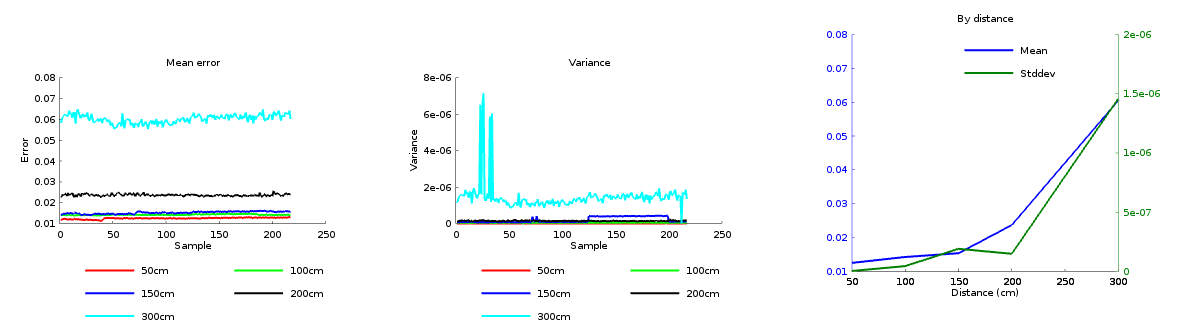
\includegraphics[width=1\textwidth]{figures/20x20-plot.png}
    \captionof{figure}[Mean and variance: 20x20 window]{\label{fig:20x20} The error and variance for a 20x20 pixel window at the center.}
  \end{figure}
  \begin{figure}[ht]
    \centering
    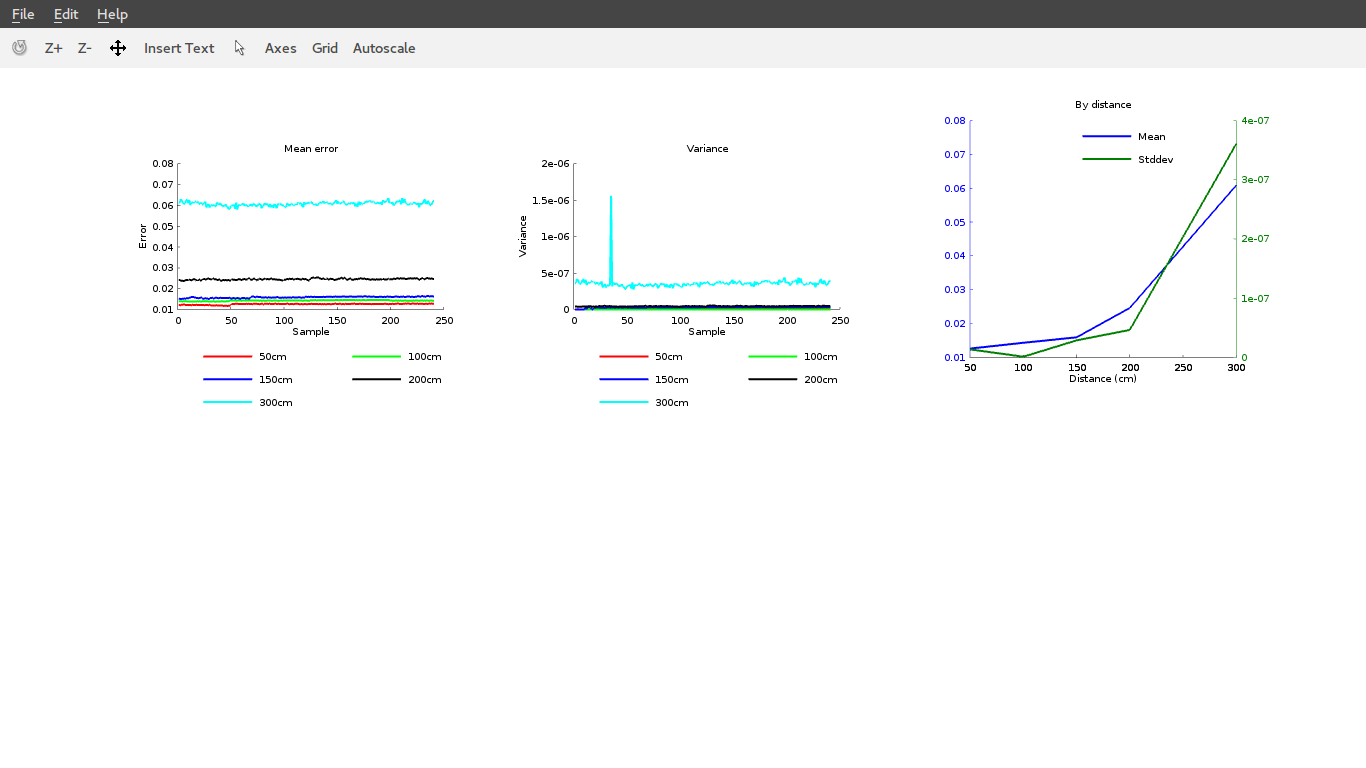
\includegraphics[width=1\textwidth]{figures/plot40x40.png}
    \captionof{figure}[Mean and variance: 40x40 window]{\label{fig:40x40} The error and variance for a 40x40 pixel window at the center.}
  \end{figure}
  \begin{figure}[ht]
    \centering
    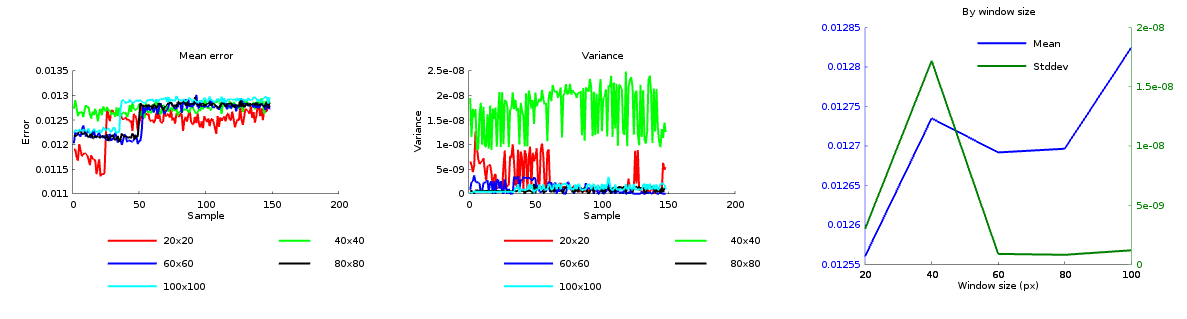
\includegraphics[width=1\textwidth]{figures/plotwindowsizes.png}
    
    \captionof{figure}[Mean and variance: 50cm, varied window sizes]{\label{fig:variedwindow} The error and variance at 50cm for various window sizes.}
  \end{figure}

% TODO: Tom : Show plots; Measuring setup;
% TODO: Both : Analysis of plots
\subsection{Noise filtering}
% TODO: Tom : Implementation, challenges (NAAAN), push code with visible images
% TODO: Marek : Target scene (point 3)
% TODO: Both : Analysis

\section{Results}
% Both : Summary...

\bibliography{References}
\end{document}



%%% Local Variables:
%%% mode: latex
%%% TeX-master: t
%%% End:
